\documentclass{article}

\usepackage[left=2cm,right=2cm, top=2cm, bottom = 2cm]{geometry}
\usepackage{amsfonts}
%%%\usepackage{array}

\usepackage{amsmath}
\usepackage{xcolor}

\usepackage{tikz}

\pagestyle{empty}

\setlength{\tabcolsep}{15pt}
%%%\renewcommand{\arraystretch}{2.5}

%%%\makeatletter
%%%\newcommand{\thickhline}{%
%%%    \noalign {\ifnum 0=`}\fi \hrule height 2pt
%%%    \futurelet \reserved@a \@xhline
%%%}
%%%\newcolumntype{!}{@{\hskip\tabcolsep\vrule width 2pt\hskip\tabcolsep}}
%%%\makeatother

\begin{document}

\title{Limits and the Small Angle Approximations}
\date{}

\maketitle
\thispagestyle{empty}

\Large

\textbf{\underline{Objective: To have an intuitive understanding of limits of functions}}

\textbf{\underline{and the algebra of limits, and the small-angle approximations for}}

\textbf{\underline{sine and cosine.}}



\vspace{5mm}


\textbf{Recap of previous material:}

\vspace{5mm}

A particle moves in a straight line. Its position $x$ at time $t$ is $x=4t^2-3t+7$.
\begin{enumerate}
	\item Find the starting position of the particle.
	\item Find the velocity of the particle at time $t$.
	\item Find the time at which the velocity is 0.
	\item Find the acceleration of the particle at time $t$.
\end{enumerate}










\clearpage

{\bf Warm-up---Small-Angle Approximations:}

\vspace{5mm}


All angles below are measured in radians.


\begin{enumerate}
	\item
		\begin{enumerate}
			\item What is the circumference of a circle of radius $r$?
			\item What is the arc length $l$ of the sector below, in terms of $r$ and $\theta$?
				\begin{center}
				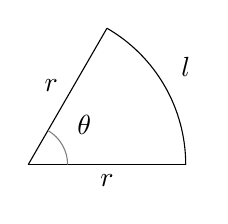
\begin{tikzpicture}
					\draw (2,0) arc (0:60:2);
					\draw (0,0) -- (2,0);
					\draw (0,0) -- (1,1.732);
					
					\node[below] at (1,0) {$r$};
					\draw[gray] (0.5,0) arc (0:60:0.5);
					\node[right] at (0.5,0.5) {$\theta$};
					\node[left] at (0.5,1) {$r$};
					\node[above] at (2,1) {$l$};
				\end{tikzpicture}
				\end{center}
		\end{enumerate}
	\item Consider the diagram below of a sector of the unit circle, in which the vertical line is perpendicular to the base radius.
		\begin{center}
		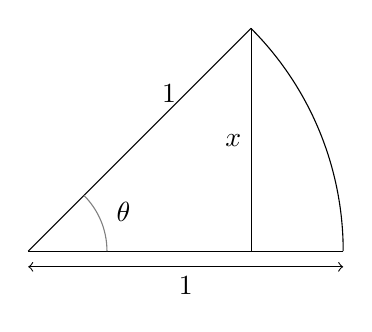
\begin{tikzpicture}
			\draw (4,0) arc (0:45:4);
			\draw (0,0) -- (4,0);
			\draw (0,0) -- (2.83,2.83);
			\draw (2.83,0) -- (2.83,2.83);
			
			\draw[gray] (1,0) arc (0:45:1);
			\node[right] at (1,0.5) {$\theta$};
			\draw[<->] (0,-0.2) -- (4,-0.2);
			\node[below] at (2,-0.2) {$1$};
			\node[left] at (2,2) {$1$};
			\node[left] at (2.83,1.4) {$x$};
		\end{tikzpicture}
		\end{center}
		
		\begin{enumerate}
			\item Write $\sin(\theta)$ in terms of $x$.
			\item Now suppose that $\theta$ is very small, so that the vertical line and the arc are almost the same length. Using your expression for the arc length from question 1, 					write an estimate of $\sin(\theta)$ for small angles.
		\end{enumerate}
	\item Consider the diagram below of a sector of the unit circle. In this diagram, the vertical line is perpendicular to the base radius, and the chord is the hypotenuse of the right-angled 				triangle thus formed to the right and has length $h$.
		\begin{center}
		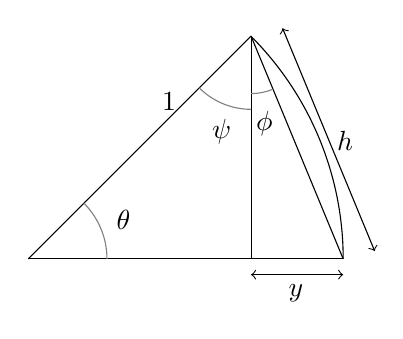
\begin{tikzpicture}
			\draw (4,0) arc (0:45:4);
			\draw (0,0) -- (4,0);
			\draw (0,0) -- (2.83,2.83);
			\draw (2.83,0) -- (2.83,2.83);
			\draw (4,0) -- (2.83,2.83);
			
			\draw[gray] (1,0) arc (0:45:1);
			\node[right] at (1,0.5) {$\theta$};
			\node[left] at (2,2) {$1$};
			\draw[<->] (2.83,-0.2) -- (4,-0.2);
			\node[below] at (3.4,-0.2) {$y$};
			\draw[<->] (4.4, 0.1) -- (3.23,2.93);
			\node[right] at (3.8, 1.5) {$h$};
			
			\draw[gray] (2.83,2.1) arc (270:292.5:0.73);
			\node[below] at (3,2) {$\phi$};
			
			\draw[gray] (2.83,1.9) arc (270:225:0.93);
			\node[below left] at (2.7,1.9) {$\psi$};
		\end{tikzpicture}
		\end{center}
		
		\begin{enumerate}
			\item Express $\cos(\theta)$ in terms of $y$.
			\item Find $\psi$ in terms of $\theta$.
			\item Hence find $\phi$ in terms of $\theta$ (hint: the two radii form an isosceles triangle).
			\item Express $y$ in terms of $\phi$ and $h$.
			\item Now suppose $\theta$ is very small, so that $h$ is approximately equal to the arc length. Using your expression for the arc length from question 1 and estimating $					\sin(\phi)$ by the method from question 2, give an estimate of $\cos(\theta)$ for small values of $\theta$.
		\end{enumerate}
\end{enumerate}

\vspace{40mm}

We thus have the following \textbf{small-angle approximations}, for small values of $\theta$ \underline{measured in radians}:
\[\sin(\theta)\approx \theta\qquad\qquad\cos(\theta)\approx 1-\frac{\theta^2}{2}.\]

It is essential that we use radians to have these approximations, as they were derived based on the formula $\mathrm{arc \;length} = r\theta$, which is only valid in radians.




\clearpage


{\bf Theory --- Limits of Functions:}

\vspace{5mm}

Fundamental to both differentiation and integration is the notion of a limit. We saw last time that the rate of change of a function $f(t)$ at time $t$ is found by considering what happens to
\[\frac{f(t+h)-f(t)}{h}\]
as $h$ gets very close to 0. To make this idea precise, we need the notion of a limit. The proper definition is that the rate of change of $f(t)$ at time $t$ is the limit of the above expression as $h$ tends to 0.\bigskip


Suppose we want to get $f(x)$ ``close to'' $L$. We can describe this more precisely by picking a small width $\epsilon$ and saying that the ``target zone'' around $L$ is from $L-\epsilon$ to $L+\epsilon$. So if $f(x)$ is within $\epsilon$ of $L$, we're ``on-target''. Then we can ask what values of $x$ will lead to us being on-target; this is our ``launch zone''.

We show below two different target zones and their corresponding launch zones. Note that in the second case, the launch zone is actually in two separate parts.

\begin{center}
\begin{tikzpicture}
	\draw[->] (0,0) -- (5,0);
	\node[right] at (5,0) {$x$};
	\draw[->] (0,0) -- (0,5);
	\node[above] at (0,5) {$y$};
	
	\draw[domain=0:5] plot (\x, {0.333*\x^3-2*\x^2+4*\x-0.01*\x^4});
	
	\draw[thin] (-0.1,2.5) -- (0.1,2.5);
	\node[right] at (0,2.5) {$L$};
	\draw[red,ultra thick] (0,2) -- (0,3);
	\draw[<->] (-0.2,2) -- (-0.2,2.5);
	\node[left] at (-0.2,2.25) {$\epsilon$};

	\node[right,red] at (-3.5,2.5) {Target zone};
	
	\draw[dotted] (0,2) -- (5,2);
	\draw[dashed] (0.742,2) -- (0.742,0);
	\draw[dotted] (0,3) -- (5,3);
	\draw[dashed] (4.156,3) -- (4.156,0);
	
	\draw[blue, ultra thick] (0.742,0) -- (4.156,0);
	\node[below,blue] at (2.4,0) {Launch zone};
	
	
	
	
	
	
	\draw[->] (7,0) -- (12,0);
	\node[right] at (12,0) {$x$};
	\draw[->] (7,0) -- (7,5);
	\node[above] at (7,5) {$y$};
	
	\draw[domain=7:12] plot (\x, {0.333*(\x-7)^3-2*(\x-7)^2+4*(\x-7)-0.01*(\x-7)^4});
	
	\draw[thin] (6.9,2.5) -- (7.1,2.5);
	\node[right] at (7,2.5) {$L$};
	\draw[red, ultra thick] (7,2.3) -- (7,2.7);
	\draw[<->] (6.8,2.3) -- (6.8,2.5);
	\node[left] at (6.8,2.4) {$\epsilon$};
	
	\draw[dotted] (7,2.3) -- (12,2.3);
	\draw[dashed] (7.977,2.3) -- (7.977,0);
	\draw[dashed] (9.533,2.3) -- (9.533,0);
	\draw[dashed] (10.542,2.3) -- (10.542,0);
	\draw[dotted] (7,2.7) -- (12,2.7);
	\draw[dashed] (10.962,2.7) -- (10.962,0);
	
	\draw[blue, ultra thick] (7.977,0) -- (9.533,0);
	\draw[blue, ultra thick] (10.542,0) -- (10.962,0);
	\node[below,blue] at (9.4,0) {Launch zone};
	
\end{tikzpicture}
\end{center}


Now, if we pick a target zone around $L$, we can ask if starting close enough to $a$ is guaranteed to put us inside the launch zone. That is, is there some small $\delta>0$ such that if we start with $x$ between $a-\delta$ and $a+\delta$, we are in the launch zone, and so $f(x)$ is in the target zone? We have to be careful though, as with $f(x)=\frac{\sin(x)}{x}$, for example, $f(0)$ is not defined. So actually we want to consider values of $x$ between $a-\delta$ and $a+\delta$, but \textbf{excluding} $a$ itself.

So our definition of the limit is this: if for any small $\epsilon>0$, there is some $\delta>0$ such that every value of $x$ between $a-\delta$ and $a+\delta$ (except $a$ itself) is in the launch zone to land in the target zone from $L-\epsilon$ to $L+\epsilon$, then $L$ is the limit of $f(x)$ as $x$ tends to $a$:
\[L=\lim_{x\to a}f(x).\]

We can write this more compactly as: for all $\epsilon>0$ there exists $\delta>0$ such that if $-\delta<x-a<\delta$ and $x\neq a$, then $-\epsilon<f(x)-L<\epsilon$.

We can use the modulus function to measure the distance between two points; $|x-a|=\sqrt{(x-a)^2+0^2}$, as $x-a$ has imaginary part zero, so this is $\sqrt{(x-a)^2}$, which is either $x-a$ or $a-x$, whichever is non-negative. So this is the distance between $a$ and $x$ on the axis. So $-\delta<x<\delta$ can be written more compactly as $|x-a|<\delta$. Similarly we can express being in the target zone by $|f(x)-L|<\epsilon$. Saying that $x\neq a$ is saying that the distance between $a$ and $x$ is not 0, so we can express that as $0<|x-a|$. So our definition of the limit can be written as:\bigskip

\noindent\fbox{\parbox{\textwidth}{The definition of
\[\lim_{x\to a}f(x)=L\]
(also written as ``$f(x)\to L$ as $x\to a$'') is that:\medskip

For all $\epsilon>0$ there exists $\delta>0$ such that if $0<|x-a|<\delta$, then $|f(x)-L|<\epsilon$.
}}\bigskip

We think of this as saying ``no matter how small a target zone we take around $L$, we can take a small launch zone around $a$ and guarantee $f(x)$ will be inside the target zone if $x$ is in this launch zone.''

\vspace{5mm}


This definition, called the $\epsilon$-$\delta$ definition of the limit, is the ``correct'' way to understand limits; however, it is difficult to apply in practice. Most of the time, a looser, more intuitive understanding of limits suffices. The idea is that as $x$ gets closer to $a$, $f(x)$ should get closer to $L$, and we can get $f(x)$ as close to $L$ as we like by getting $x$ close enough to $a$; in most situations, this intuitive idea will not lead you astray. However, it is important to be aware of the $\epsilon$-$\delta$ definition, and to know that if you ever have a problem with limits, the answer lies in the $\epsilon$-$\delta$ definition (though it can be very hard to extract!).

From now on we will work with an intuitive notion of limits, and establish some important results in this way. At the end of this sheet, proper proofs of these results using the $\epsilon$-$\delta$ definition are provided. You should look at these at least once, to get some idea of how the definition is applied in practice, but you shouldn't dwell on them too much---the value you get from them won't be worth the time it would take to fully understand them!

\clearpage

\textbf{Example:}\bigskip



We have seen from our small angle approximations that $\sin(x)\approx x$ for small values of $x$, and this approximation gets more accurate the smaller $x$ is; so $\frac{\sin(x)}{x}\approx\frac{x}{x}$ for small $x$, and gets closer the smaller $x$ gets. So
\[\lim_{x\to 0}\frac{\sin(x)}{x}=1.\]

A proper proof of this from the $\epsilon$-$\delta$ definition is much harder, and is given in the tricky stuff at the end.\bigskip


\clearpage









\textbf{Theory---The Algebra of Limits:}

\vspace{5mm}

A key result in the study of limits is the \textbf{algebra of limits}, which tells us how to combine functions whose limits we know. It has three parts. In all three, we assume that $f(x)$ and $g(x)$ are functions, and that as $x\to a$, $f(x)\to F$ and $g(x)\to G$.
\begin{enumerate}
	\item \[\lim_{x\to a}[f(x)+g(x)]=F+G\]
	\item \[\lim_{x\to a}[f(x)g(x)] = FG\]
	\item If $G\neq 0$, then \[\lim_{x\to a}\left[\frac{f(x)}{g(x)}\right]=\frac{F}{G}.\]
\end{enumerate}

So limits behave as nicely as we could hope when adding, multiplying, or dividing functions, with the usual caveat that we must be careful not to divide by 0. We will give an intuitive explanation of why these results are true:

\begin{enumerate}
	\item To show that $f(x)+g(x)\to F+G$, we take a target zone around $F+G$ of width $\epsilon$. Then we can take a target zone around $F$ of width $\frac{\epsilon}{2}$, and one around $G$ again of width $\frac{\epsilon}{2}$. Because $f(x)\to F$, we can take a launch zone around $a$ which puts $f(x)$ inside our target zone around $F$, and similarly there is a launch zone putting $g(x)$ inside the target zone around $G$. Then when $x$ is inside both of these launch zones, $f(x)$ is within $\frac{\epsilon}{2}$ of $F$ and $g(x)$ is within $\frac{\epsilon}{2}$ of $G$, so $f(x)+g(x)$ is within $\epsilon$ of $F+G$, as required. Essentially, if $f(x)$ is close to $F$ and $g(x)$ is close to $G$, then $f(x)+g(x)$ must be close to $F+G$.
	\item To show that $f(x)g(x)\to FG$ is a little harder, though intuitively it should still be clear that if $f(x)$ is close to $F$ and $g(x)$ is close to $G$, $f(x)g(x)$ will be close to $FG$. The problem is that knowing how close $f(x)$ is to $F$ and $g(x)$ is to $G$ doesn't directly tell us how close $f(x)g(x)$ is to $FG$; for instance, if $f(x)=F=1000$, and $g(x)=G-0.1$, then $f(x)g(x)=F(G-0.1)=FG-100$, which is quite far from $FG$. Of course, we can always make $g(x)$ closer still to $G$, but this shows that we need to be more careful about this.
	
	So the trick is to first get $Fg(x)$ close to $FG$, then get $f(x)g(x)$ close to $Fg(x)$; this way, we only need to worry about one of the functions at a time. So take a target zone of width $\epsilon$ around $FG$ and a target zone of width $\frac{\epsilon}{2F}$ around $G$ (assuming $F\neq 0$---have a think about what to do if $F=0$!). Then we can take a launch zone around $a$ such that if $x$ is in this launch zone, $g(x)$ is within $\frac{\epsilon}{2F}$ of $G$, so $Fg(x)$ is within $\frac{\epsilon}{2}$ of $FG$.
	
	Now we have $Fg(x)$ close to $FG$, so let's get $f(x)g(x)$ close to $Fg(x)$. The problem with doing this is that the size of $g(x)$ could vary a lot. But we know we can get $g(x)$ close to $G$, so we can take a launch zone around $a$ in which $g(x)$ never gets far from $G$, and so never gets bigger than some $M$ which is slightly bigger than $G$. Then we can take a target zone around $F$ of width $\frac{\epsilon}{2M}$, and a launch zone around $a$ that puts $f(x)$ inside this target zone, so then $f(x)g(x)$ is within $\frac{\epsilon}{2M}g(x)$ of $Fg(x)$; since $g(x)$ is smaller than $M$ within this launch zone, that means $f(x)g(x)$ is within $\frac{\epsilon}{2}$ of $Fg(x)$.
	
	So now we have a launch zone in which $f(x)g(x)$ is within $\frac{\epsilon}{2}$ of $Fg(x)$ and $Fg(x)$ is within $\frac{\epsilon}{2}$ of $FG$, so $f(x)g(x)$ is within $\epsilon$ of $FG$. So $f(x)g(x)\to FG$, as claimed.
	
	\item The proof of this result is harder, and we won't actually need it, so we'll skip it. A rigorous proof is provided at the end though, with the rest of the tricky stuff!
\end{enumerate}












\clearpage


{\bf Key Points to Remember:}

\vspace{5mm}

\begin{enumerate}
\item For small angles $\theta$, $\sin(\theta)\approx \theta$ and $\cos(\theta)\approx 1-\frac{\theta^2}{2}$.
\item If for any target zone around a number $L$ we can take a launch zone around $a$ such that if $x$ is in this launch zone, then $f(x)$ is in the target zone, then we say that $f(x)\to L$ as $x\to a$.
\item \[\frac{\sin(x)}{x}\to 1 \mbox{ as } x\to 0.\]
\item If $f(x)$ and $g(x)$ are functions, and $f(x)\to F$, $g(x)\to G$ as $x\to a$, then
	\begin{enumerate}
		\item $f(x)+g(x)\to F+G$.
		\item $f(x)g(x)\to FG$.
		\item If $G\neq 0$ $\frac{f(x)}{g(x)}\to \frac{F}{G}$.
	\end{enumerate}
\end{enumerate}




\clearpage









\textbf{\LARGE Using the $\epsilon$-$\delta$ definition to calculate a limit and prove key results:}\bigskip






\textbf{Example of calculating a limit:}

\vspace{5mm}

\textbf{Warning: this section is difficult! Don't expect to understand it the first time reading---or even the second or third. A summary is provided at the end, to help you keep track of the steps in the argument.}

\vspace{5mm}


We have already argued intuitively that $\frac{\sin(x)}{x}$ should be roughly 1 when $x$ is small. Now that we have a precise definition of limits, we can prove this. We want to show that for any $\epsilon>0$ there exists a $\delta>0$ such that if $0<|x|<\delta$, then $\left|\frac{\sin(x)}{x}-1\right|<\epsilon$. 

We will show that
\[\left|\frac{\sin(x)}{x}-1\right|\leq\frac{x^2}{2};\]
this is difficult, so on first reading skip the section in red and focus on the rest of the argument. Then you can come back and read about how we show this once you understand everything else.\medskip

{\color{red}


Consider the following diagram:


\begin{center}
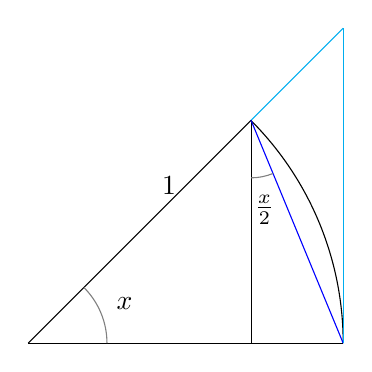
\begin{tikzpicture}
	\draw (4,0) arc (0:45:4);
	\draw (0,0) -- (4,0);
	\draw (0,0) -- (2.83,2.83);
	\draw[cyan] (2.83,2.83) -- (4,4);
	\draw (2.83,0) -- (2.83,2.83);
	\draw[blue] (4,0) -- (2.83,2.83);
	\draw[cyan] (4,0) -- (4,4);
	
	\draw[gray] (1,0) arc (0:45:1);
	\node[right] at (1,0.5) {$x$};
	\node[left] at (2,2) {$1$};

	
	\draw[gray] (2.83,2.1) arc (270:292.5:0.73);
	\node[below] at (3,2) {$\frac{x}{2}$};
\end{tikzpicture}
\end{center}

The vertical red line has length $|\sin(x)|$, whereas the vertical cyan line has length $|\tan(x)|$; the absolute value bars are included to allow $x$ to be negative. Since the area of a triangle is given by half the base times the height, the triangle with the blue side opposite $x$ has area $\frac{1}{2}|\sin(x)|$, while the area of the triangle with the cyan side opposite $x$ is $\frac{1}{2}|\tan(x)|$. Contained between those two triangles is the sector of the unit circle, whose area is
\[\frac{\pi |x|}{2\pi}=\frac{|x|}{2}.\]
Therefore we have
\[\frac{|\sin(x)|}{2}\leq \frac{|x|}{2}\leq \frac{|\tan(x)|}{2}.\]
Multiplying through by $2$ and dividing by $|\sin(x)|$, we get
\[1\leq \frac{|x|}{\sin(x)}\leq \frac{1}{|\cos(x)|}.\]
Taking reciprocals of both sides:
\[1\geq \frac{|\sin(x)|}{|x|}\geq|\cos(x)|.\]

Now we observe that for $\frac{-\pi}{2}<x<\frac{\pi}{2}$, and $x\neq 0$, $\sin(x)$ and $x$ have the same sign, while $\cos(x)$ is positive. So we can drop the absolute value bars to find
\[1\geq\frac{\sin(x)}{x}\geq\cos(x).\]
Subtracting 1 from these inequalities, we obtain
\[0\geq \frac{\sin(x)}{x}-1\geq\cos(x)-1.\]
Now we use our small angle approximation for cosine, which tells us that $\cos(x)\geq 1-\frac{x^2}{2}$. Substituting this in and taking absolute values, we conclude that
\[0\leq \left|\frac{\sin(x)}{x}-1\right|\leq\frac{x^2}{2}.\]
}

So
\[0\leq \left|\frac{\sin(x)}{x}-1\right|\leq\frac{x^2}{2}.\]

Now, if we want to get $\left|\frac{\sin(x)-x}{x}\right|<\epsilon$, it is sufficient to get $\frac{x^2}{2}<\epsilon$. If we take $|x|<\sqrt{2\epsilon}$, then $|x|^2<2\epsilon$, so $\frac{x^2}{2}<\epsilon$, and hence
\[\left|\frac{\sin(x)}{x}-1\right|\leq\frac{x^2}{2}<\epsilon.\]
So we take $\delta=\sqrt{2\epsilon}$, and conclude that if $0<|x|<\delta$, then $|f(x)-1|<\epsilon$, and this works for any $\epsilon>0$. So
\[\lim_{x\to 0}\frac{\sin(x)}{x} = 1.\]

\vspace{5mm}

\textbf{Summary:}\medskip

We want to show that $\frac{\sin(x)}{x}\to 1$ as $x\to 0$. By the definition of a limit, this means we need to show that for any $\epsilon>0$, there is a $\delta>0$ such that if $0<|x|<\delta$, then $|f(x)-1|<\epsilon$. Unwrapping this, this means that we need to show no matter how narrow our target zone around 1 is, we can guarantee to be inside our launch zone if we start with $x$ close enough to 0 (closer than $\delta$).

To do this, we show that $|f(x)-1|\leq \frac{x^2}{2}$, and hence we can make $|f(x)-1|$ land inside our target zone as long as we can make $\frac{x^2}{2}$ land in the target zone. But Starting with $x$ in a launch zone from $-\sqrt{2\epsilon}$ to $\sqrt{2\epsilon}$ will guarantee this. So no matter how small our target zone, we can find a suitable launch zone.\bigskip















\clearpage


\textbf{Theory---the Algebra of Limits:}\medskip

\textbf{Warning: hard!}\medskip


Let $f(x)$ and $g(x)$ be two functions, such that $f(x)\to F$ and $g(x)\to G$ as $x\to a$ (for some numbers $a$, $F$, and $G$). We will show that $f(x)+g(x)\to F+G$ as $x\to a$.

By the definition of the limit, this means we need to show that for any $\epsilon>0$ (target zone), we can make sure that $|f(x)+g(x)-F-G|<\epsilon$ (we're in the target zone) by starting from $x$ closer to $a$ than $\delta$ (in the launch zone). So fix our $\epsilon>0$, and let's find our $\delta$.

Since we know that $f(x)\to F$ as $x\to a$, we can take any target zone we like around $F$ and get $f(x)$ within that target zone. Let's take a target zone from $F-\frac{\epsilon}{2}$ to $F+\frac{\epsilon}{2}$; then there exists some $\delta_f$ such that if $|x-a|<\delta_f$, $f(x)$ will be within the target zone: $|f(x)-F|<\frac{\epsilon}{2}$.

Similarly, $g(x)\to G$ as $x\to a$, so we can take the same size target zone around $G$ and find some $\delta_g$ such that if $|x-a|<\delta_g$, then $g(x)$ is in the target zone: $|g(x)-G|<\frac{\epsilon}{2}$.

Now let's take $\delta$ to be the smaller out of $\delta_f$ and $\delta_g$, so that if $x$ is within $\delta$ of $a$, it must be both within $\delta_f$ of $a$ and within $\delta_g$ of $a$---so it's in both launch zones! So for $|x-a|<\delta$, we're in the launch zones for both $f$ and $g$, so $|f(x)-F|<\frac{\epsilon}{2}$ and $|g(x)-G|<\frac{\epsilon}{2}$. Therefore
\[|f(x)+g(x)-F-G| \leq |f(x)-F|+|g(x)-G|<\frac{\epsilon}{2}+\frac{\epsilon}{2}=\epsilon.\]

So by starting within $\delta$ of $a$, we've made $f(x)+g(x)$ within $\epsilon$ of $F+G$. This will work no matter what $\epsilon$ we picked to start with, so we've proved that $f(x)+g(x)\to F+G$ as $x\to a$.\bigskip


So we've shown that if $f(x)$ and $g(x)$ are any two functions, and
\[\lim_{x\to a}f(x)=F\qquad\mbox{ and }\qquad \lim_{x\to a}g(x)=G,\]
then
\[\lim_{x\to a}[f(x)+g(x)] = F+G.\]

\bigskip

This proof was given with a lot of explanation. A more concise form of the proof is:\medskip

{\color{red}
Fix $\epsilon>0$. Since $f(x)\to F$, there exists some $\delta_f>0$ such that if $|x-a|<\delta_f$, then $|f(x)-F|<\frac{\epsilon}{2}$. Similarly, since $g(x)\to G$, there exists some $\delta_g>0$ such that if $|x-a|<\delta_g$, then $|g(x)-G|<\frac{\epsilon}{2}$. Let $\delta$ be the smaller of $\delta_f$ and $\delta_g$; then if $|x-a|<\delta$, $|f(x)+g(x)-F-G|\leq |f(x)-F|+|g(x)-G|<\frac{\epsilon}{2}+\frac{\epsilon}{2}=\epsilon$.
}

\clearpage





\textbf{Theory---the Algebra of Limits (cont.):}\medskip

\textbf{Warning: hard!}\medskip

Let $f(x)$ and $g(x)$ be two functions, such that $f(x)\to F$ and $g(x)\to G$ as $x\to a$ (for some numbers $a$, $F$, and $G$). We will show that $f(x)g(x)\to FG$ as $x\to a$.

First we deal with the case when $G=0$. In this case, we need to show that $f(x)g(x)\to )$. First take a target zone of width 1 around $F$; then there is a launch zone around $a$ from which $f(x)$ is within $1$ of $F$; in particular, $|f(x)|< |F|+1$. Now take a target zone of width $\epsilon$ around $0$, and a target zone around $G$ of width $\frac{\epsilon}{|F|+1}$. Then there is a launch zone around $a$ in which $g(x)$ is closer to $G$ than $\frac{\epsilon}{|F|+1}$, and $|f(x)|<|F|+1$, so $|f(x)g(x)|<(|F|+1)\frac{\epsilon}{|F|+1}=\epsilon$. So we have found a launch zone in which $f(x)g(x)$ is closer to 0 than $\epsilon$, so $f(x)g(x)\to 0$.\medskip

So we have dealt with the case $G=0$, and can now treat the case where $G$ is non-zero. We need to show that for any $\epsilon>0$ (target zone), we can make sure that $|f(x)g(x)-FG|<\epsilon$ (we're in the target zone) by starting from $x$ closer to $a$ than $\delta$ (in the launch zone). So fix our $\epsilon>0$, and let's find our $\delta$.

We'll use a cunning trick:
\begin{align*}
	f(x)g(x)-FG&=f(x)g(x)-f(x)G+f(x)G-FG\\
	&= f(x)(g(x)-G)+(f(x)-F)G.
\end{align*}
The first part of this we can deal with using the fact that $g(x)\to G$, and the second part using the fact that $f(x)\to F$.


Since $f(x)\to F$, we can take a target zone around $F$ of width $\frac{\epsilon}{2|G|}$ (note: since we've already dealt separately with the case $G=0$, we are now only concerned with $G\neq 0$, so dividing by $|G|$ is fine). Then there is some $\delta_f$ such that if $x$ is in a launch zone from $a-\delta_f$ to $a+\delta_f$, then $f(x)$ is in the target zone around $F$, so $|f(x)-F|<\frac{\epsilon}{2|G|}$, and so $|(f(x)-F)G|<\frac{\epsilon}{2|G|}|G|=\frac{\epsilon}{2}$. This deals with the $(f(x)-F)G$ term in the above expression.

For the $f(x)(g(x)-G)$ term, we have the problem that $f(x)$ could vary in size. But we can force $f(x)$ to be close to $F$; so let $M=|F|+\frac{\epsilon}{2|G|}$; then if $|x-a|<\delta_f$, we know that $F-\frac{\epsilon}{2|G|}<f(x)<F+\frac{\epsilon}{2|G|}$, so $|f(x)|<M$. Now we set our target zone around $G$ to be from $G-\frac{\epsilon}{2M}$ to $G+\frac{\epsilon}{2M}$ and take $\delta$ small enough to force us inside there, and also smaller than $\delta_f$ (since we need that to make sure $f$ is bounded by $M$).

Now if $|x-a|<\delta$, we have $|f(x)|<M$ and $|g(x)-G|<\frac{\epsilon}{2M}$, so
\[|f(x)(g(x)-G)|<M\frac{\epsilon}{2M}<\frac{\epsilon}{2},\]
and also
\[|f(x)-F|G<\frac{\epsilon}{2}\]
from the previous working. So
\[|f(x)g(x)-FG|\leq |f(x)(g(x)-G)| + |(f(x)-F)G| <\frac{\epsilon}{2}+\frac{\epsilon}{2}=\epsilon.\]

So if we start with $x$ within $\delta$ of $a$, then $f(x)g(x)$ lands within $\epsilon$ of $FG$. So we've proved:\bigskip

So we've shown that if $f(x)$ and $g(x)$ are any two functions, and
\[\lim_{x\to a}f(x)=F\qquad\mbox{ and }\qquad \lim_{x\to a}g(x)=G,\]
then
\[\lim_{x\to a}[f(x)g(x)] = FG.\]

\bigskip

Again, this was a very wordy explanation of the proof. The proof itself can be expressed as:\medskip

{\color{red}
Fix $\epsilon>0$. First suppose $G=0$; then there exists some $\delta_f>0$ such that if $|x-a|<\delta_f$, then $|f(x)-F|<1$, so $|f(x)|<|F|+1$, and there exists some $\delta_g>0$ such that if $|x-a|<\delta_g$, then $|g(x)|<\frac{\epsilon}{|F|+1}$. Let $\delta$ be the smaller of $\delta_f$ and $\delta_g$; then if $|x-a|<\delta$, $|f(x)g(x)|<(|F|+1)\frac{\epsilon}{|F|+1}=\epsilon$, so $f(x)g(x)\to 0=FG$. So if $G=0$, we're done.

Now suppose $G\neq 0$. Since $f(x)\to F$, there exists some $\delta_f>0$ such that if $|x-a|<\delta_f$, then $|f(x)-F|<\frac{\epsilon}{2|G|}$, so $|f(x)G-FG|<|G|\frac{\epsilon}{2|G|}=\frac{\epsilon}{2}$. Let $M=|F|+\frac{\epsilon}{2|G|}$, so for $|x-a|<\delta_f$, $|f(x)|<M$. Take $\delta_g>0$ such that if $|x-a|<\delta_g$, then $|g(x)-G|<\frac{\epsilon}{2M}$. Let $\delta$ be the smaller of $\delta_f$ and $\delta_g$; then if $|x-a|<\delta$, we have
\begin{align*}
	|f(x)g(x)-FG| &= |f(x)g(x)-f(x)G+f(x)G-FG|\\
	&\leq |f(x)g(x)-f(x)G|+|f(x)G-FG|\\
	&<\frac{\epsilon}{2}+M\frac{\epsilon}{2M}\\
	&=\epsilon.
\end{align*}

So $f(x)g(x)\to FG$, as claimed.
}

\clearpage










\textbf{Theory---the Algebra of Limits (cont.):}\medskip

\textbf{Warning: hard!}\medskip


Let $g(x)$ be a function such that $g(x)\to G\neq 0$ as $x\to a$. We shall prove that $\frac{1}{g(x)}\to \frac{1}{G}$ as $x\to a$. We shall give first the concise proof, then a short explanation.\medskip

{\color{red}
Fix $\epsilon>0$. Take $\delta_1>0$ such that if $|x-a|<\delta_1$, then $|g(x)-G|<\frac{|G|}{2}$, so $|g(x)|>\frac{|G|}{2}$, and so $\frac{1}{|g(x)|}<\frac{2}{|G|}$. Now take $\delta_2>0$ such that if $|x-a|<\delta_2$, then $|g(x)-G|<\epsilon\frac{|G|^2}{2}$. Now let $\delta$ be the smaller of $\delta_1$ and $\delta_2$; then if $|x-a|<\delta$, we have
\begin{align*}
	\left|\frac{1}{g(x)}-\frac{1}{G}\right| &=\frac{|g(x)-G|}{|g(x)G|}\\
	&< \frac{2|g(x)-G|}{|G|^2}\\
	&< \frac{2\epsilon|G|^2}{2|G|^2}\\
	&= \epsilon.
\end{align*}

So $\frac{1}{g(x)}\to \frac{1}{G}$ as $x\to a$, as required.
}

\bigskip


So the idea is that we treat $\frac{1}{g(x)}-\frac{1}{G}$ as $\frac{G-g(x)}{g(x)G}$. We can make $g(x)$ close to $G$, but the $g(x)$ in the denominator is a problem. So we choose a launch zone that gets $g(x)$ between $G-\frac{G}{2}$ and $G+\frac{G}{2}$, so $|g(x)|>\frac{|G|}{2}$. Then we have $\frac{1}{|g(x)|}<\frac{2}{|G|}$, so we can replace the varying $g(x)$ in the denominator with the constant $\frac{|G|}{2}$, so now $\frac{1}{g(x)}-\frac{1}{G}$ ``looks like'' $\frac{2(g(x)-G)}{|G|G}$.

Now we take a target zone of width $\frac{\epsilon|G|^2}{2}$, so we can take a launch zone around $a$ which makes $g(x)$ closer to $G$ than $\frac{\epsilon|G|^2}{2}$, and hence within both this and the previous launch zone, we have the sequence of inequalities above, showing that $\frac{1}{g(x)}$ is within $\epsilon$ of $\frac{1}{G}$.










\end{document}